% IEEE standard conference template; to be used with:
%   spconf.sty  - LaTeX style file, and
%   IEEEbib.bst - IEEE bibliography style file.
% --------------------------------------------------------------------------
\documentclass[letterpaper]{article}
\usepackage{algpseudocode}
\usepackage{algorithm}
\usepackage{spconf,amsmath,amssymb,graphicx}
\usepackage[space]{grffile}
\usepackage{epstopdf}
\usepackage{graphicx}
\usepackage[section]{placeins}

% Example definitions.
% --------------------
% nice symbols for real and complex numbers
\newcommand{\R}[0]{\mathbb{R}}
\newcommand{\C}[0]{\mathbb{C}}

% bold paragraph titles
\newcommand{\mypar}[1]{{\bf #1.}}

% Title.
% ------
\title{Minimum Spanning Tree: a parallel approach}


% For example:
% ------------
%\address{School\\
%		 Department\\
%		 Address}
%
% Two addresses (uncomment and modify for two-address case).
% ----------------------------------------------------------
\twoauthors
  {Th. Cambier, R. Dang-Nhu, Th. Dardinier}
  {
	Ecole Polytechnique\\
  	{\small Route de Saclay, 91128 Palaiseau Cedex, FRANCE}\\
  	ETH Z\"urich, D-INFK\\
	{\small R\"amistrasse 101, 8092 Z\"urich, SWITZERLAND}
  }
  {C. Trassoudaine\sthanks{The fourth author performed the work while at ETH Z\"rich}}
  {
	  IMT Atlantique,\\
	  {\small 655 Avenue du Technopôle, 29280 Plouzané, FRANCE}\\
	  EURECOM, Data Science dpt.,\\
	  {\small 450 route des Chappes, 06410 Biot, FRANCE}
  }


\begin{document}
%\ninept
%
\maketitle
%


\begin{abstract}

Many efficient algorithms have been designed to find the minimum spanning tree in connected graphs as this problem is at the heart of a broad scope of real-life applications and other graph theory problems. 
In this paper we present our implementations of algorithms already present in the literature as well as a new algorithm, Filter Sollin, which combines ideas from Filter Kruskal and parallel implementations of Sollin's algorithm. All the algorithms are tested through the EULER cluster on various benchmarks (dense graphs, sparse graphs and real-life graphs) and compared to the baseline from the Parallel Boost Graph Library.

\textbf{Keywords:} Minimum spanning tree, distributed algorithms, high performance computing cluster 


\end{abstract}

\section{Introduction}\label{sec:intro}

A wide range of problems have input sets that can be represented as graphs which is why it is crucial to develop efficient graph algorithms to reduce the computation costs. As graphs are getting larger and larger, classic sequential algorithms are becoming not fast enough to cope with the exploding number of nodes and edges. To further reduce costs, distributed algorithms are ideal to take advantage of the parallel architecture of computers but it is a challenge to correctly handle memory, concurrency or security and one needs to understand parallel software and hardware to design algorithms that scale well.
In this paper, we focus on the minimum spanning tree problem which is a classical one in graph theory with applications in network design, cluster analysis or the approximation of NP-hard problems such as the travelling salesman problem. 

We implemented five algorithms. Two of them are based on Kruskal's sequential implementation and the other three on Sollin's and we present here the runtimes and speedups we obtained when running them over various benchmarks on the High Performance Computing cluster EULER (Section \ref{sec:setup}). 

All our code can be found on our project repository on GitHub at \cite{code}.

\mypar{Related work} The implementations of our algorithms are based upon the works presented in several previously published papers.
In \cite{kruskal} is described an implementation of the Filter Kruskal algorithm that we present in Section \ref{sec:parKruskal}.
In \cite{sollin} are described several parallel implementations of Sollin's algorithm and, notably, Bor-AL and Bor-FAL that we present in Section \ref{sec:parSollin} under the names Sollin AL and Sollin AL. Our implementations of these algorithms iare also based upon techniques presented in \cite{pointerJump}. Both \cite{kruskal} and \cite{sollin} were an inspiration when we designed a new algorithm, Filter Sollin that combines the filtering steps from Filter Kruskal and Sollin's parallel implementation (Section \ref{sec:parSollin}).


\section{Minimum Spanning Tree and sequential algorithms}\label{sec:background}

In this section, we formally define the Minimum Spanning Tree (MST) problem and introduce the main sequential algorithms upon which are based the parallel implementations of Section \ref{sec:algo}.

\mypar{Minimum Spanning Tree}
A minimum spanning tree is a subset of the edges of a connected, edge-weighted undirected graph that connects all the vertices together, without any cycles and with the minimum possible total edge weight.
That is, it is a spanning tree whose sum of edge weights is as small as possible. 
Here we consider only undirected and connected graphs and we present different algorithms to compute the minimum spanning tree over them. 

In the following, we will use V to denote the set of vertices of the graph, E for the set of edges, n for the number of vertices and m for the number of edges.

\mypar{MST sequential algorithms} The three main sequential algorithms to compute minimum spanning trees are Prim's, Kruskal's and Sollin's (also known as Bor\r{u}vka)  algorithms. All are greedy approaches :
\begin{itemize}
    \item Prim : we initialise a tree with a single random vertex and, at each step, we choose the vertex connected to the tree with the smallest-weighted edge and add it to the tree until all vertices are added.
    \item Kruskal : we sort the edges of the graph by increasing weight and, at each step, we add to the tree the smallest edge that does not create a cycle.
    \item Sollin : we initialise each vertex of the graph as a set and, at each step, we add the smallest-weighted edge from every set to another until the tree is formed.
\end{itemize}

Prim's algorithm computes a minimum spanning tree in $\mathcal{O}(mlog(n))$ when implemented with adjacency list representation and a binary heap to keep the vertices sorted by the smallest weight from an edge that connects them to any vertex in the partially constructed tree.

Kruskal's algorithm (Algorithm \ref{algo:kruskal}) relies on an union-find data structure which maintains a set for each connected component. If we want to add an edge with its extremities in different components, we need to merge the components because they are now connected. The sorting of the edges is done in $\mathcal{O}(mlog(m))$ sequentially and the adding of edges is done in $\mathcal{O}(m)$.

Sollin's algorithm takes $\mathcal{O}(log(n))$ iterations until it terminates because they are V components at the beginning and each iteration reduces the number of components by at least two. Therefore it runs in time $\mathcal{O}(mlog(n))$.

\begin{algorithm}
\caption{kruskal}
\label{algo:kruskal}
\begin{algorithmic}
\State U is the Union-Find structure
\State sort E by increasing weight
\For {${u,v} \in E$}
    \If {u and v are in different components in U}
        \State add ${u,v}$ to the tree
        \State join u and v representations in U
    \EndIf
\EndFor

\end{algorithmic}
\end{algorithm}


\section{Parallel Algorithms}\label{sec:algo}

In this section, we present the parallel algorithms that we implemented for computing the minimum spanning tree in a connected graph.
In the following p is the number of cores on which the parallel algorithms are run.

\subsection{Parallel Kruskal} \label{sec:parKruskal}

We implemented two parallel versions of Kruskal's algorithm presented in Section \ref{sec:background}.

\mypar{Kruskal with parallel sorting} Kruskal's algorithm is inherently sequential as it linearly goes through the edges once these ones have been sorted. Thus, our first implementation of Kruskal's algorithm is the sequential algorithm described in Algorithm \ref{algo:kruskal} preceded by a parallel sorting using TBB (Section \ref{sec:setup}).

\mypar{Filter Kruskal} The second parallel MST algorithm we consider is a variant of Kruskal's algorithm that is named Filter Kruskal (Algorithm \ref{algo:filterKruskal}).

The idea of this algorithm is to "filter out" some edges that are assumed not part of the MST to reduce sorting time.
Firstly, the number of edges is compared to a threshold under which we choose to compute the sequential Kruskal.
Then, an edge is chosen as a pivot regarding weight to separate the edges in two weight categories (heavier and lighter edges).
A first recursive call is made on the lighter edges and, before making the second recursive call on the heavier ones, all heavy edges that are within a component of the current forest are removed (filtering step).
To finish the algorithm, the results from both calls are merged to form the MST.

In our implementation, the edges are kept in a vector and elements are permuted in-place, as in a quick-sort, without requiring additional amounts of memory which leads to maximal operational intensity. Moreover, the filter and partition functions are both implemented with the partition function from the C++ standard library parallelised with Parallel STL (Section \ref{sec:setup}).

\begin{algorithm}
\caption{filterKruskal}
\label{algo:filterKruskal}
\begin{algorithmic}
\If {$m\leq threshold$}
    kruskal
\Else
    \State find pivot $p \in E$
    \State partition E in $E_{\leq}, E_{>}$
    \State $A_{\leq} = filterKruskal(E_{\leq})$
    \State $E_{>} = filter(E_{>})$
    \State $A_{>} = filterKruskal(E_{>})$
    \State \Return $merge(A_{\leq},  A_{>})$
\EndIf  
    
\end{algorithmic}
\end{algorithm}


For the cost analysis of the algorithm, we use $T(m)$ for the runtime of the algorithm with m edges. The choosing of the pivot can be done in $\mathcal{O}(1)$ by sampling 256 edges from the graph using OpenMP and taking the median thanks to Intel TBB (see experimental setup in Section \ref{sec:setup}).
The partition of the edges as well as the filtering can both be done in $\mathcal{O}(\frac{m}{p})$ using the partition function from Intel Parallel STL. The first recursive call costs $T(\frac{m}{2})$ and the second one $\mathcal{O}(T(\frac{m}{2}))$ (and far less in practice) because edges have been removed.
In the best case, the first recursive call is sufficient to compute the MST and we have $T(m) \leq  \mathcal{O}(\frac{m}{p}) + T(\frac{m}{2})) $ which gives $T(m) = \mathcal{O}(\frac{m}{p} + m) = \mathcal{O}(m)$.
In the worst case, we have $T(m) \leq  \mathcal{O}(\frac{m}{p}) + 2T(\frac{m}{2})) $ which gives $T(m) = \mathcal{O}(\frac{mln(m)}{p} + m)$


\subsection{Parallel Sollin} \label{sec:parSollin}

From the three greedy approaches presented in Section \ref{sec:background}, Sollin's algorithm is the one that is the most suitable to a parallel adaptation. Here are presented three distributed variants of Sollin's algorithm : Sollin AL, Sollin FAL and Filter Sollin. All of them are constituted of the same four main steps, iterated until the tree is fully grown :
\begin{itemize}
    \item Sort the adjacency lists.
    \item Merge connected components in a super-vertex.
    \item Find the edge with minimum weight for each vertex.
    \item Identify connected components.
\end{itemize}

Super-vertices are represented thanks to the Union-Find structure already used for Kruskal's algorithm (Section \ref{sec:background}). The finding of the edge of minimum weight is done concurrently with OpenMP and the connected components) identification is done via pointer-jumping according to \cite{pointerJump}.

\mypar{Sollin AL} The name Sollin AL comes from the fact that the graph is represented with adjacency lists : a vector keeps for each vertex the list of its incident edges. The vertex array is sorted according to the super-vertex label which leads the vertices with the same super-vertex to be nearby in the array allowing these vertices to be merged efficiently. Then, the adjacency lists are copied in vectors which are more cache-friendly as they allow to avoid false sharing \cite{cache} and these vectors are sorted concurrently based on the target super-vertex (the super-vertex at the other end of the edge).  Thus, self-loops and multiple edges are moved to consecutive locations to be merged.

\mypar{Sollin FAL} This time, the adjacency lists are replaced by flexible adjacency lists to reduce the cost from sorting before merging the connected components. The flexible adjacency lists are linked lists of adjacency lists composed of the adjacency lists of all the vertices with the same super-vertex : each time we perform the merging step for the connected components, we append the adjacency list of each vertex to their super-vertex adjacency list. Thus, this time, super-vertices keep multiple edges and self-loops in their adjacency lists which simplifies the sorting steps. These edges are now removed during the finding of the edge of minimum weight.

\mypar{Filter Sollin} Filter Sollin uses the approach already seen in the algorithm Filter Kruskal (Section \ref{sec:parKruskal}) but uses Sollin's algorithm (with the data structure seen in Sollin FAL) instead of Kruskal's when the input size is under a given threshold.


\section{Experimental Results}\label{sec:exp}

In this section, we present the results of our algorithms on various input sets and discuss their performance against the baselines over different benchmarks.

\subsection{Experimental setup} \label{sec:setup}

All experiments are run through the EULER cluster on an Hewlett-Packard XL230k Gen10 equipped with two 18-core Intel Xeon Gold (6150 processors, 2.7-3.7 GHz) and 192 GB of DDR4 memory clocked at 2666 MHz. We are using C++17 with GCC v5.2.0, CMake v3.11.4 and OpenMPI v1.6.5. Our algorithms are compiled with the optimisation flag O3. We also use the following dependencies :

\mypar{OpenMP} OpenMP which is an API that supports shared memory multiprocessing programming in C++.

\mypar{TBB} Threading Building Blocks (TBB) for the sorting function that takes full advantage of multi-core performance.

\mypar{PSTL} Parallel STL (PSTL) to have a threaded and vectorized execution of the standard C++ partition function, optimised and validated for Intel(R) 64 processors.

\mypar{LSB} LibSciBench (LSB) which is a framework containing a performance measurement library for parallel applications and is coupled with an R script for the post-processing of the gathered data \cite{benchmarking} \cite{measuring}. 


\subsection{Input Sets}
The experiments have been performed on the three following input sets :

\mypar{ER} Erd\H{o}s-R\'{e}nyi (ER) random graphs where we specify the number of nodes of the graph and the probability of existence of a vertex between every pair of nodes. The probability is chosen greater than $\frac{ln(n)}{n}$ which is the threshold to have almost surely a connected graph.

\mypar{PA} Preferential Attachment (PA) graphs where we specify the number of nodes of the graphs and the number of neighbours that a node attaches itself to when added in the graph. In order to have a connected graph, the graph is initialised with three connected vertices and new vertices are added one by one and connected to existing vertices with higher probability for the ones with higher degrees. This type of graph models better existing inputs from the real world such as representations of social network connections.  

\mypar{USA} USA road networks from 9th Implementation DIMACS Challenge dataset which are real input sets from the road networks in various part of the USA. These graphs are connected and undirected.

\subsection{Benchmarks}

We tested our algorithms on three benchmarks :

\mypar{Dense graphs} Around 10K nodes and 10M edges with the topology of PA or ER.

\mypar{Sparse graphs} Around 50K nodes and 2.5M edges with the topology of PA or ER.

\mypar{USA graphs} Around 300K nodes and 800K edges with the topology of the USA road networks dataset.


We also used a benchmark of smaller graphs with the topology of PA with either 1000 nodes and 100K edges or 2000 nodes and 40K edges to compare our algorithms to the baseline.

\subsection{Baselines} \label{sec:baseline}

We compare the results of our algorithms to those of the Parallel Boost Graph Library (PBGL) v1.62.0 which is an extension of the BGL for distributed computing.


\subsection{Results} We present here the results of our experiments on the benchmarks that we studied For every experiment, we generated a large number of random graphs on which three runs were made for each in order to have an appropriate standard deviation.

\mypar{Baselines} On Figures \ref{baseline1} and \ref{baseline2} are represented the runtimes of our algorithms in comparison to the ones from the baseline algorithms (Section \ref{sec:baseline}). We see that Filter Kruskal is 5 to 10 times faster than the fastest algorithm from PBGL, Sollin FAL and Filter Sollin have similar runtime and Sollin AL is slower (especially on the dense PA graph).

\begin{figure}\centering
  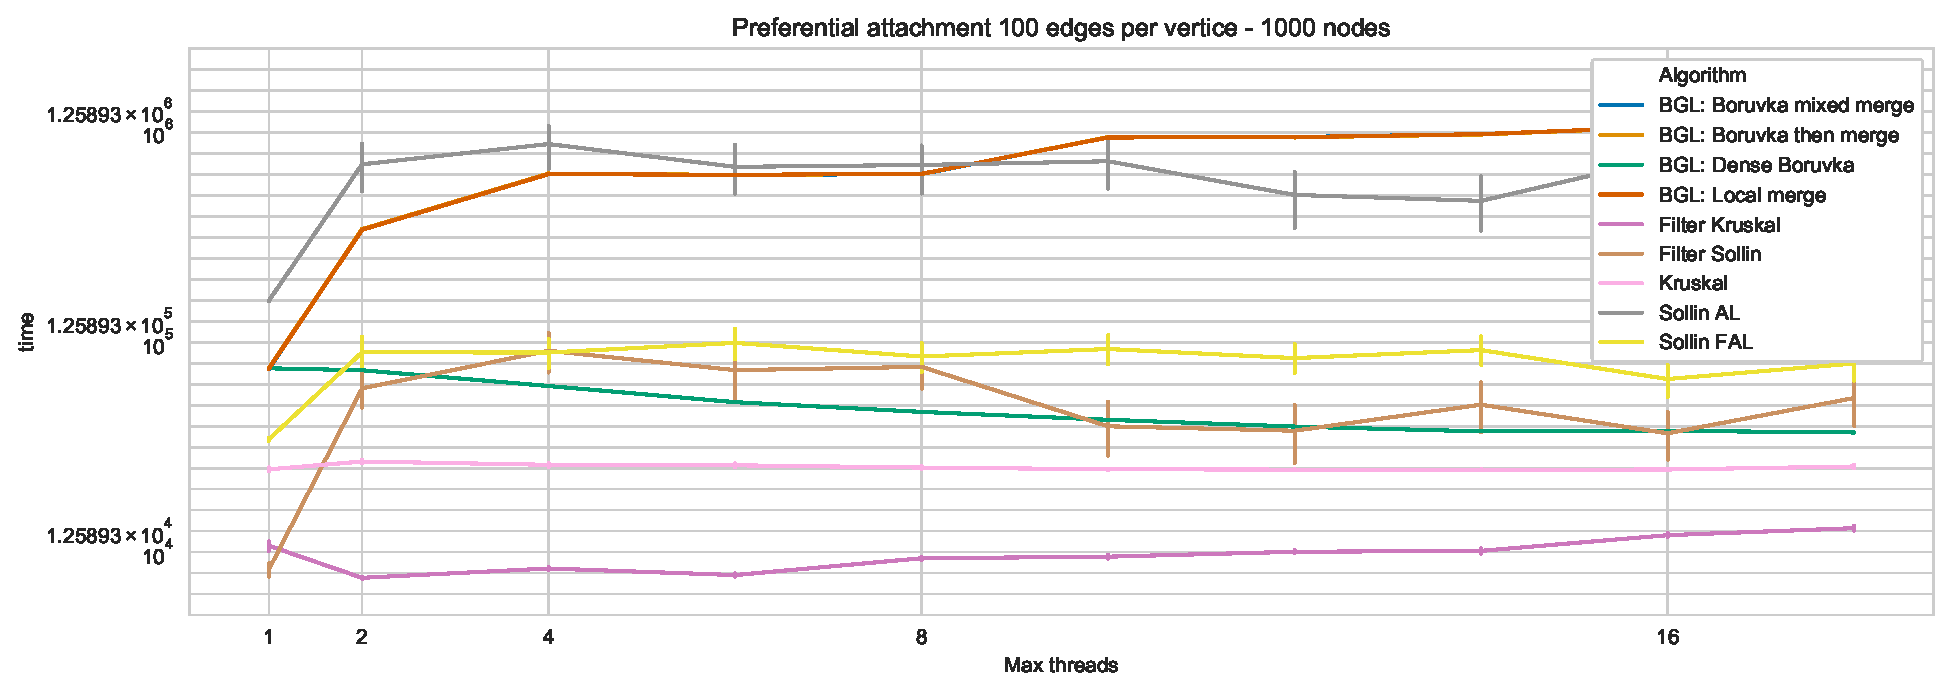
\includegraphics[width=\linewidth]{graphics/Graph_runtime_Preferential_attachment_100_edges_per_vertice_1000.eps}
  \caption{Runtime graph on PA(1 000, 100)\label{baseline1}}
\end{figure}

\begin{figure}\centering
  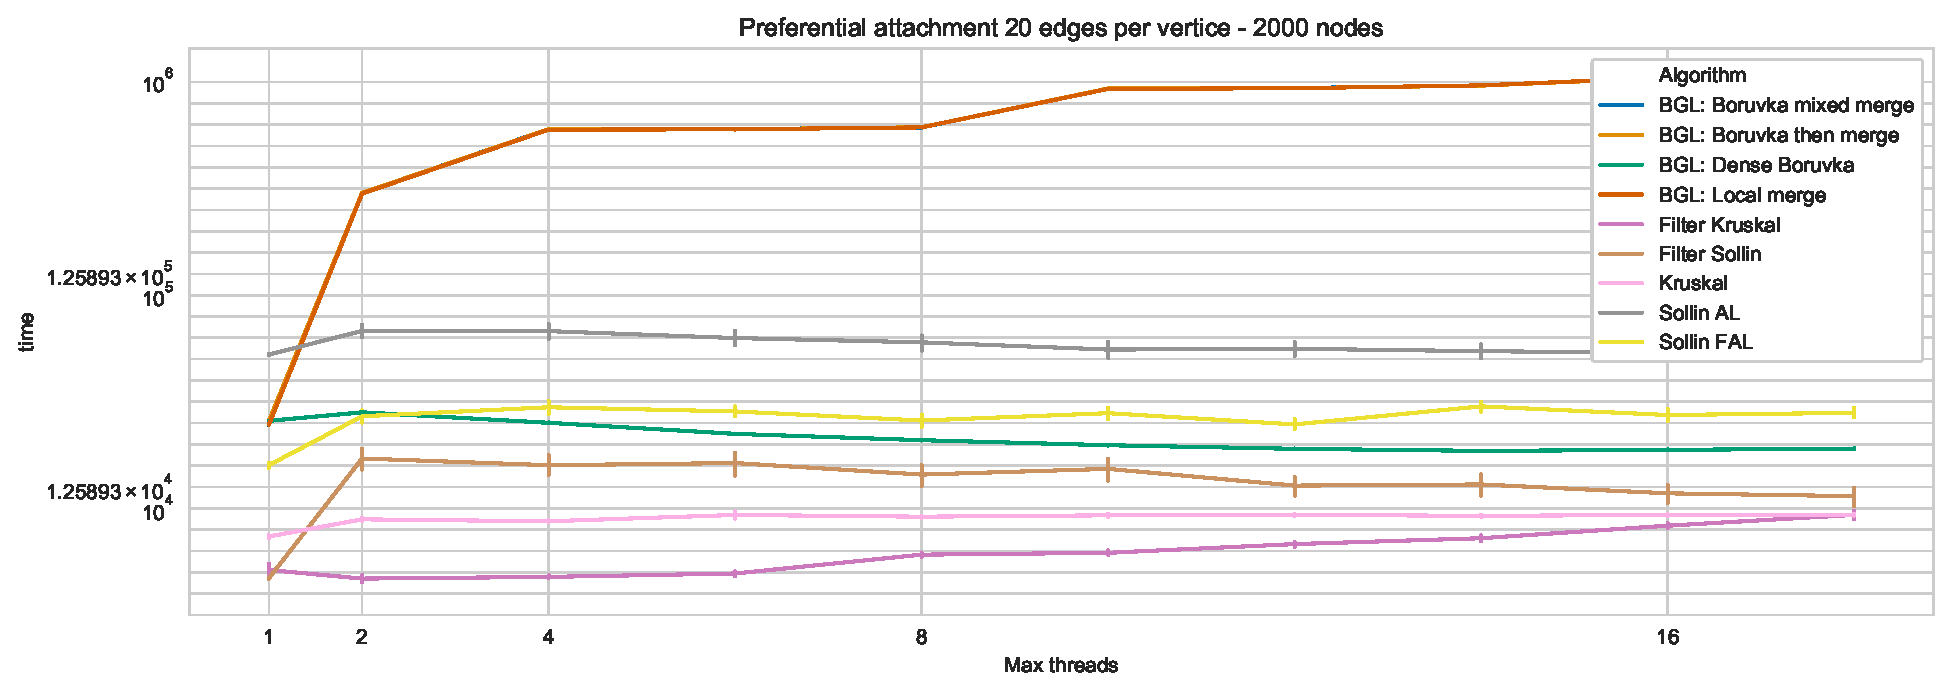
\includegraphics[width=\linewidth]{graphics/Graph_runtime_Preferential_attachment_20_edges_per_vertice_2000.eps}
  \caption{Runtime graph on PA(2 000, 20)\label{baseline2}}
\end{figure}

\mypar{Dense graphs} On dense graphs (Figures \ref{denseERruntime}, \ref{denseERspeedup}, \ref{densePAruntime} and \ref{densePAspeedup}), we see that Filter Kruskal has globally the better speedup, even reaching a speedup of 6 for 20 threads on ER graphs (Figure \ref{denseERspeedup}). On the same random graphs, we observe that Sollin FAL also shows a good scaling with a speedup greater than 6 for 28 threads or more. However, when we look at Figure \ref{denseERruntime}, we see that Filter Kruskal is more than three times faster than Sollin FAL. This is because in the implementation of Sollin FAL we have large adjacency lists which are equally distributed. Thus, the scaling works well but the initial sorting of the lists is very time consuming. On these inputs, Sollin AL behaves rather poorly : it does not scale well and it is more than 10 times slower than Filter Kruskal. We notice that on Figure \ref{denseERspeedup}, the speedup for Sollin AL decreases after reaching 18 threads due to the larger overhead of using the network (the processors have 18 cores). From Figures \ref{densePAruntime} and \ref{densePAspeedup}, we see that the trends on PA graphs are the same for the algorithms : Filter Kruskal followed by Filter Sollin are the fastest algorithms and Sollin AL the slowest. However, the speedup values are lesser than for the ER graphs because PA graphs are far less equally distributed : some nodes have a huge amount of neighbours whereas others only have one. As each thread treats nodes that are loaded differently, it is logical to see a drop in the speedup.

\begin{figure}\centering
  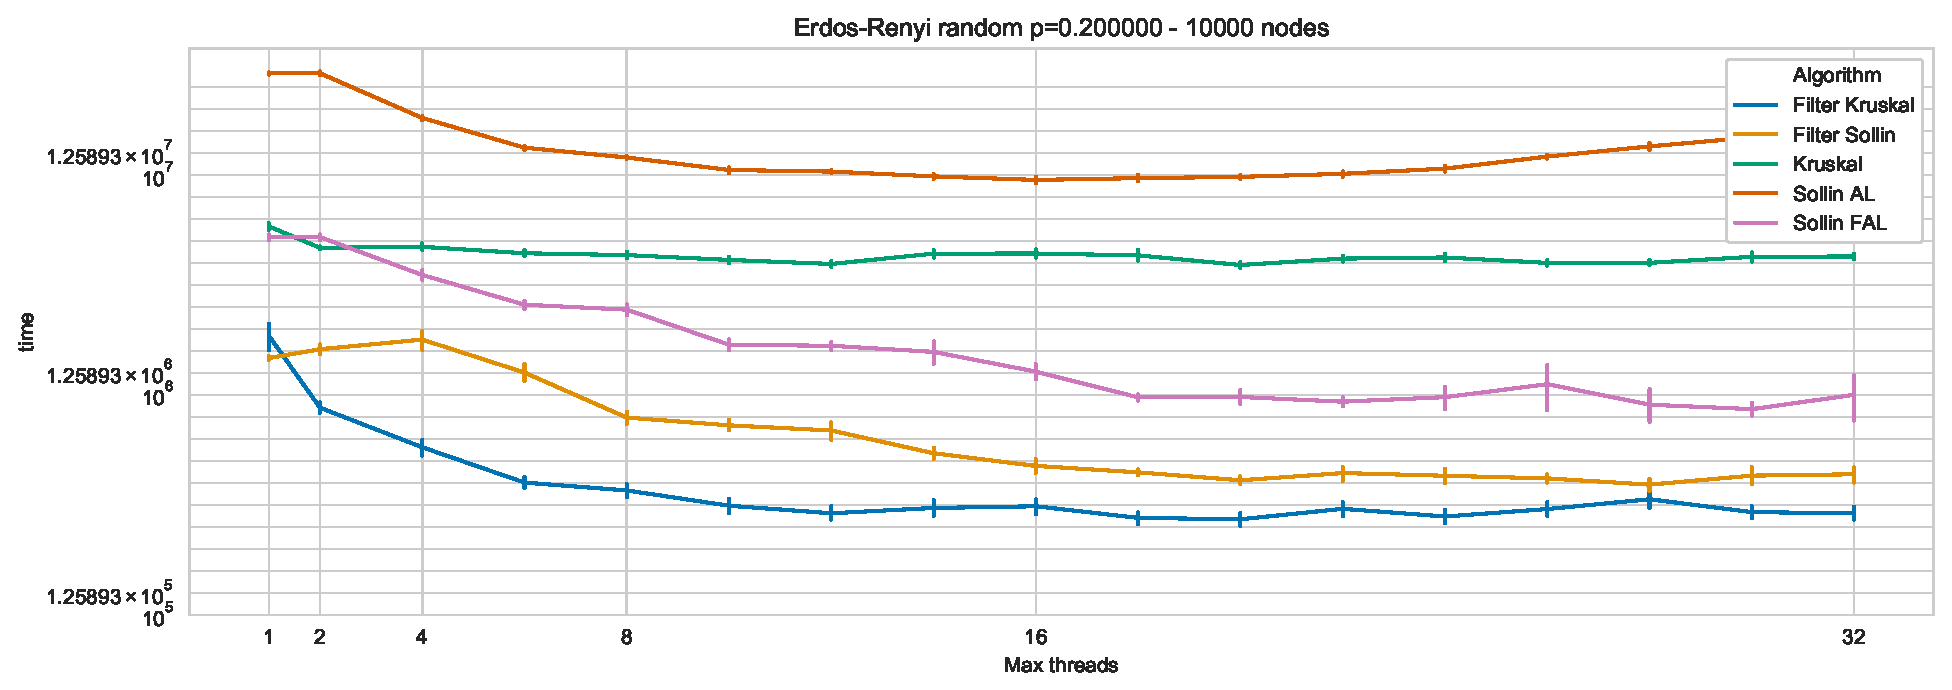
\includegraphics[width=\linewidth]{graphics/Graph_runtime_Erdos-Renyi_random_p=0.200000_10000.eps}
  \caption{Runtime graph on ER(10 000, 2 000)\label{denseERruntime}}
\end{figure}

\begin{figure}\centering
  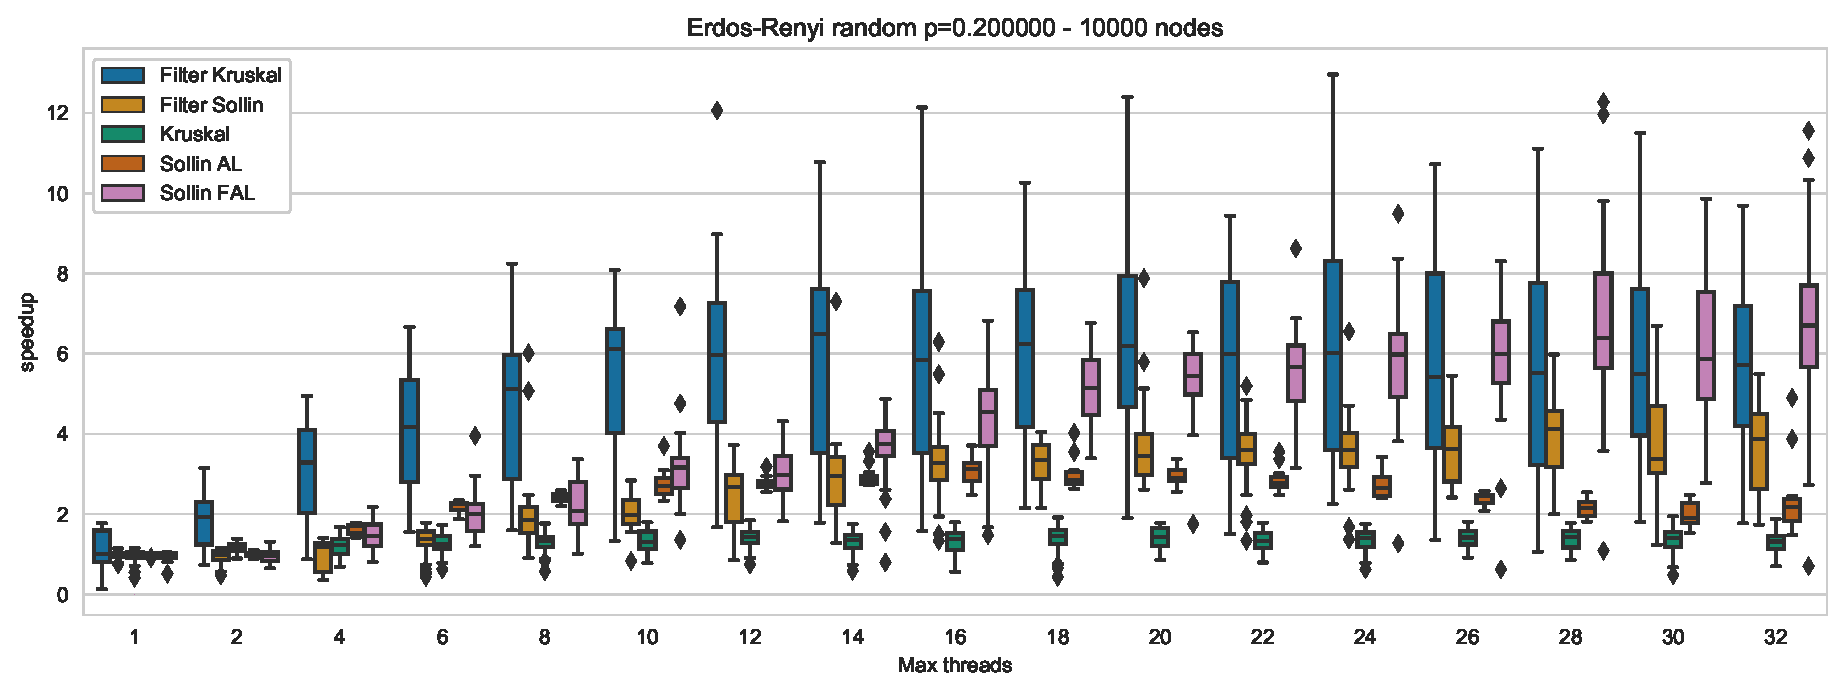
\includegraphics[width=\linewidth]{graphics/Box_Speedup_Erdos-Renyi_random_p=0.200000_10000.eps}
  \caption{Speedup graph on ER(10 000, 2 000)\label{denseERspeedup}}
\end{figure}

\begin{figure}\centering
  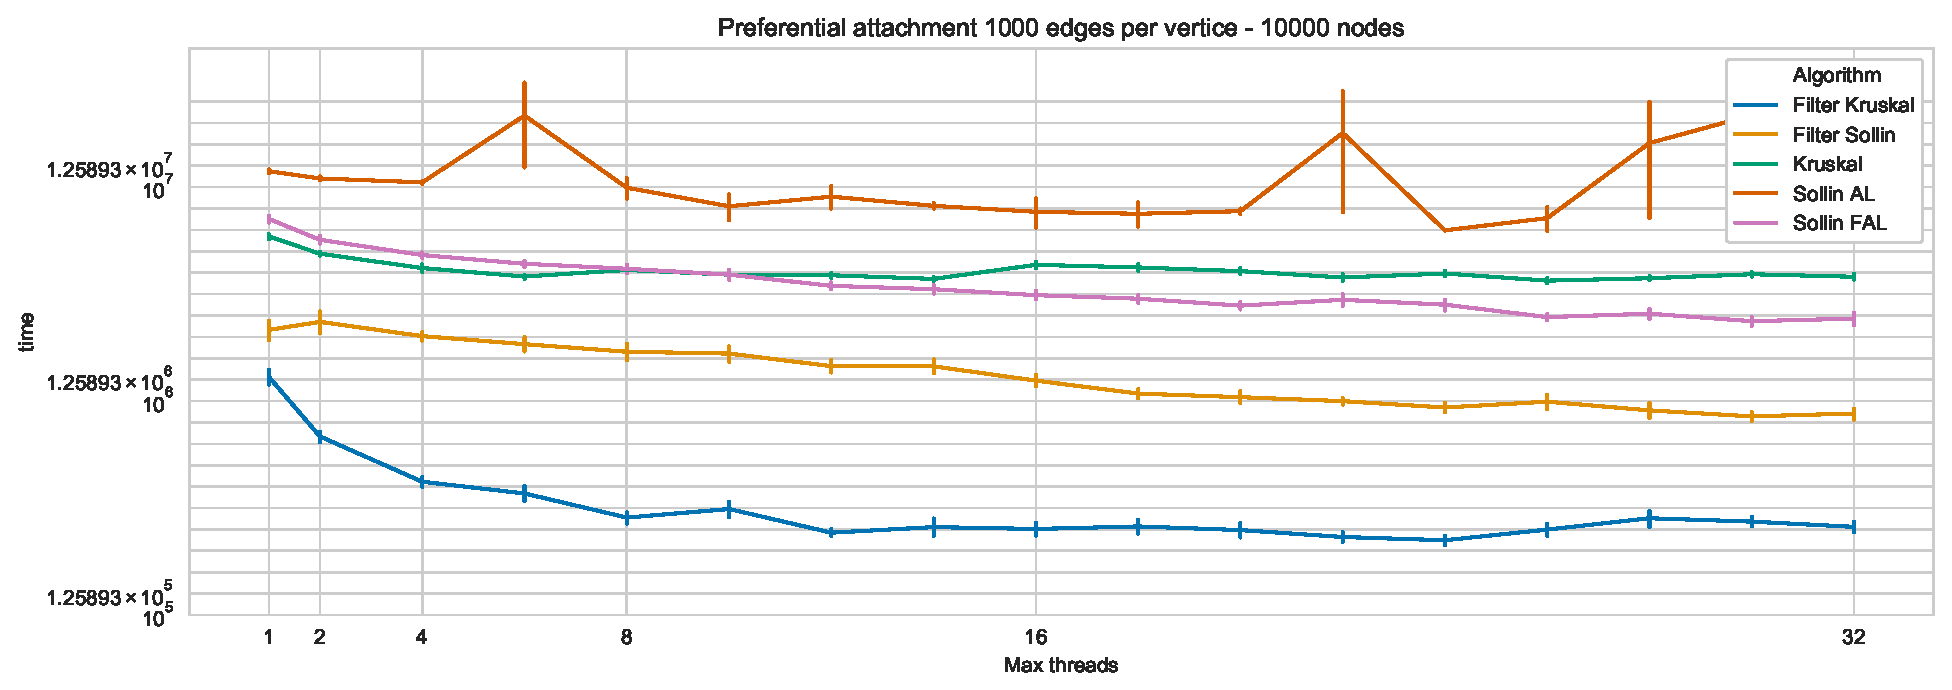
\includegraphics[width=\linewidth]{graphics/Graph_runtime_Preferential_attachment_1000_edges_per_vertice_10000.eps}
  \caption{Runtime graph on PA(10 000, 1 000)\label{densePAruntime}}
\end{figure}

\begin{figure}\centering
  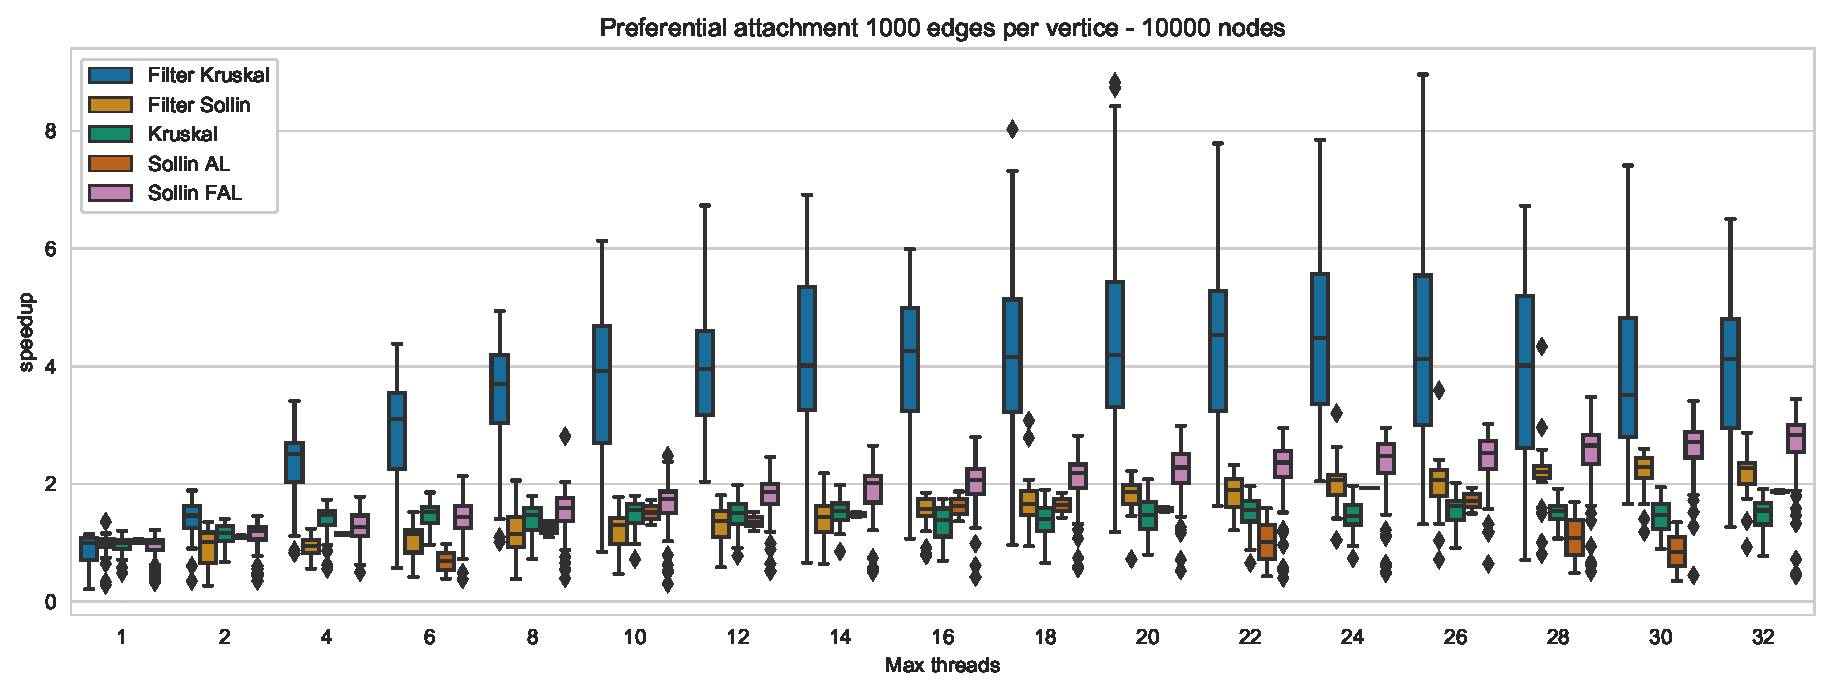
\includegraphics[width=\linewidth]{graphics/Box_Speedup_Preferential_attachment_1000_edges_per_vertice_10000.eps}
  \caption{Speedup graph on PA(10 000, 1 000)\label{densePAspeedup}}
\end{figure}



\mypar{Sparse graphs} On sparser graphs (Figures \ref{sparseERruntime}, \ref{sparseERspeedup}, \ref{sparsePAruntime} and \ref{sparsePAspeedup}), Sollin AL has a very good parallelism, reaching a speedup of 5 for 30 threads on ER graphs and Filter Kruskal and Sollin FAL also scales pretty well. However, when looking at Figure \ref{sparseERruntime}, we see that Filter Kruskal is 10 times faster than Sollin FAL and 30 times faster than Sollin AL. As with the dense graphs, the speedups on PA graphs are inferior than the ones on ER graphs but the difference is slighter because the disparity between high-degree and low-degree nodes is smaller. We also note that Filter Sollin does not scale well on either type on inputs but is still the second fastest algorithm after Filter Kruskal. On sparse graphs, the different parallel implementations of Sollin's algorithm are dominated by the step of finding the edge of minimun weight for each vertex.

\begin{figure}\centering
  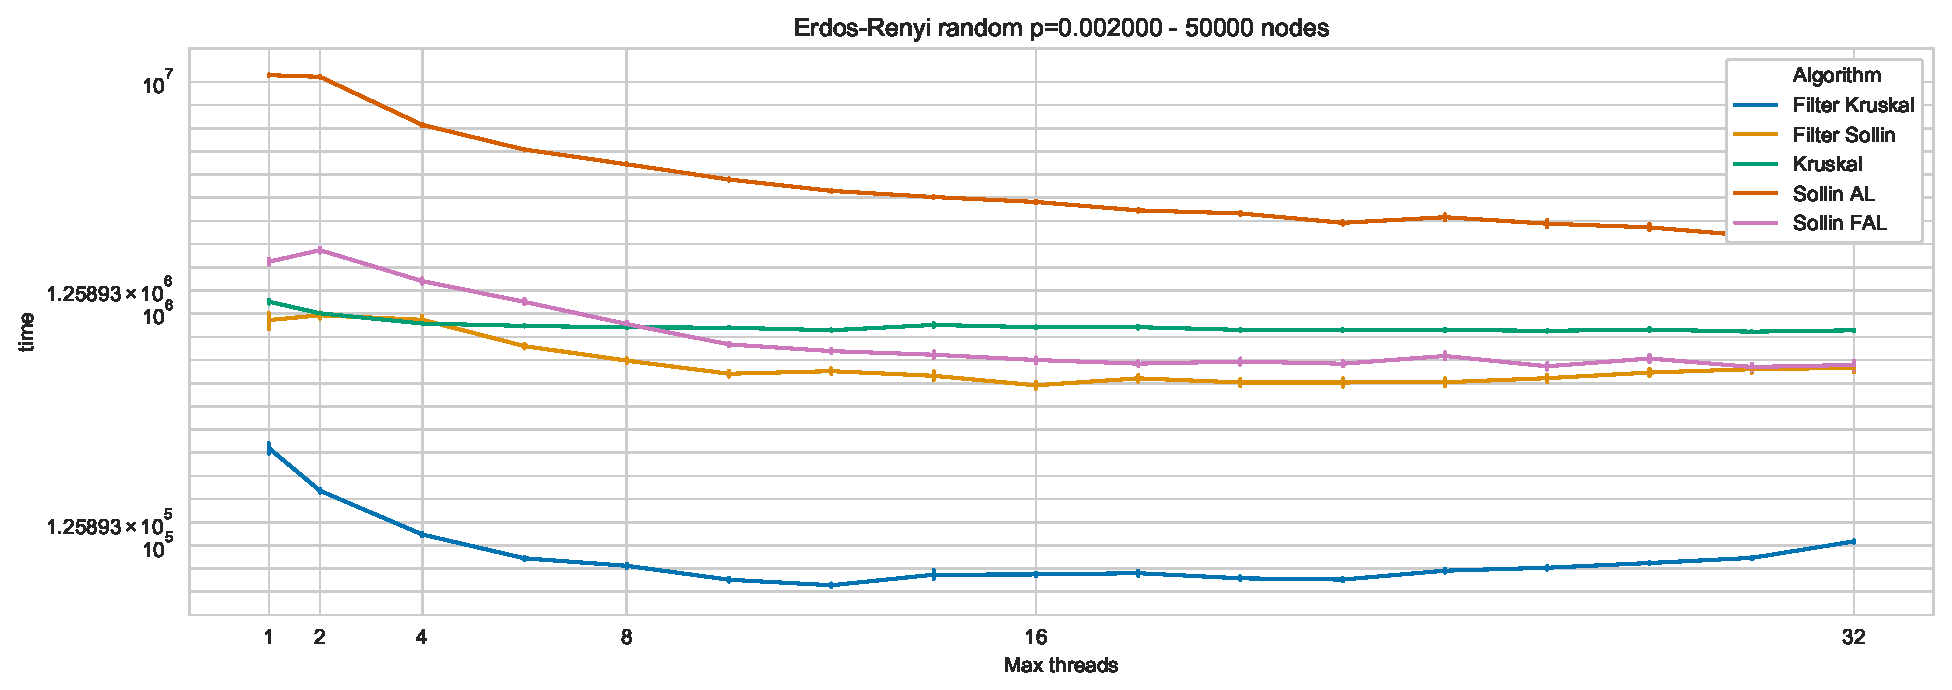
\includegraphics[width=\linewidth]{graphics/Graph_runtime_Erdos-Renyi_random_p=0.002000_50000.eps}
  \caption{Runtime graph on ER(50 000, 100)\label{sparseERruntime}}
\end{figure}

\begin{figure}\centering
  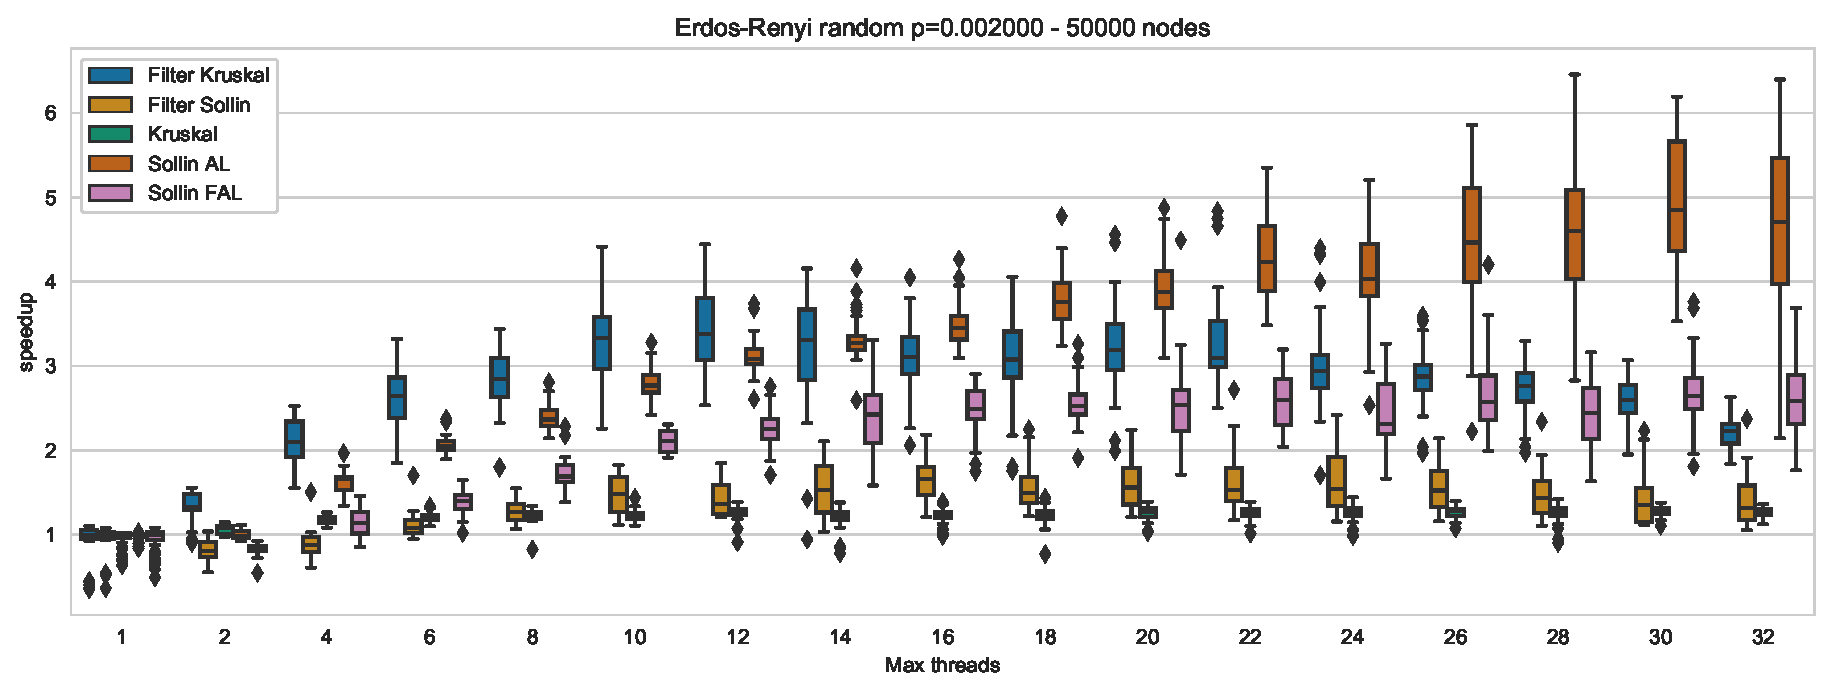
\includegraphics[width=\linewidth]{graphics/Box_Speedup_Erdos-Renyi_random_p=0.002000_50000.eps}
  \caption{Speedup graph on ER(50 000, 100)\label{sparseERspeedup}}
\end{figure}

\begin{figure}\centering
  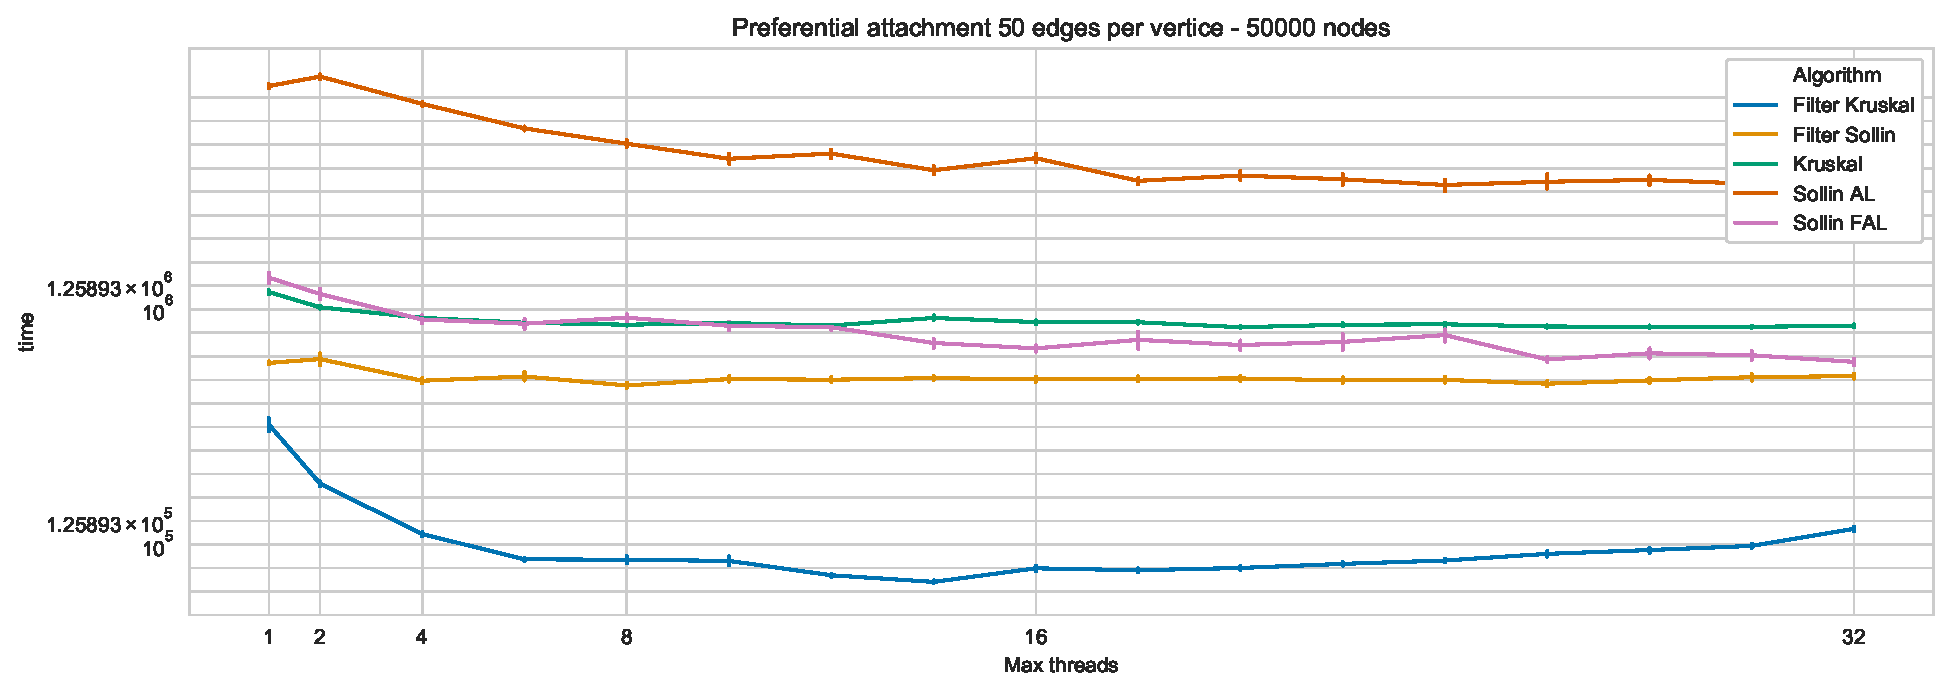
\includegraphics[width=\linewidth]{graphics/Graph_runtime_Preferential_attachment_50_edges_per_vertice_50000.eps}
  \caption{Runtime graph on PA(50 000, 50)\label{sparsePAruntime}}
\end{figure}

\begin{figure}\centering
  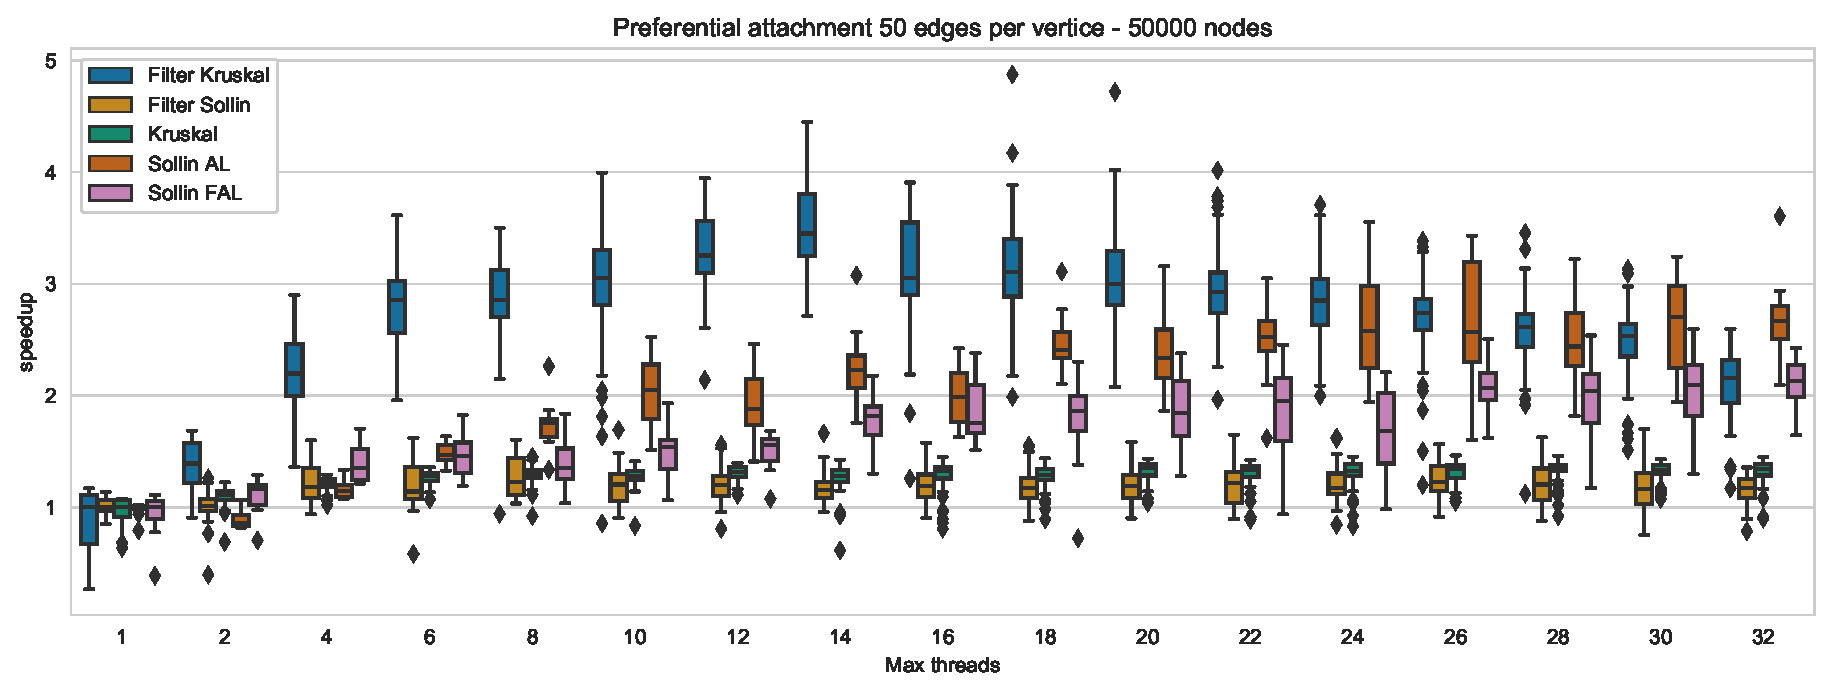
\includegraphics[width=\linewidth]{graphics/Box_Speedup_Preferential_attachment_50_edges_per_vertice_50000.eps}
  \caption{Speedup graph on PA(50 000, 50)\label{sparsePAspeedup}}
\end{figure}

\mypar{USA graphs} USA graphs give far worse results. On both Figures \ref{usaBAYspeedup} and \ref{usaNYspeedup}, we see that the algorithms do not scale at all. Only Filter Sollin shows the beginning of a scaling but it is fast outgrowed by the overhead in the parallelisation process. The topology of USA graphs does not fit well with our algorithms. From Figures \ref{usaBAYruntime} and \ref{usaNYruntime}, we observe that the Kruskal's algorithm with a parallel sorting is the fastest and is nearly 50 times faster than Filter Sollin.

\begin{figure}\centering
  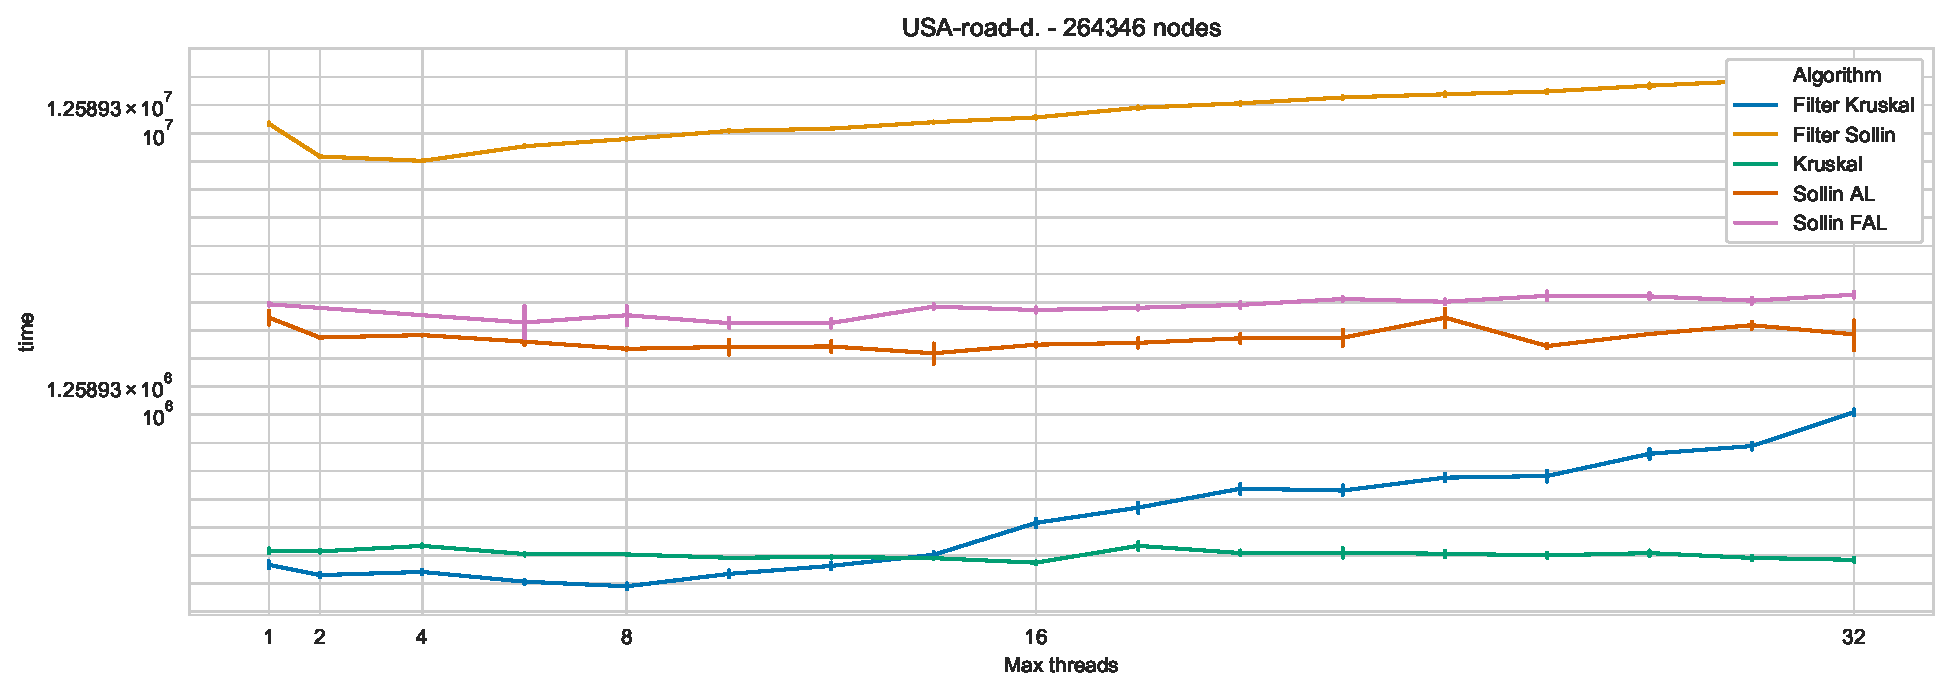
\includegraphics[width=\linewidth]{graphics/Graph_runtime_USA-road-d._264346.eps}
  \caption{Runtime graph on USA NY (260K nodes, 730K edges)\label{usaNYruntime}}
\end{figure}

\begin{figure}\centering
  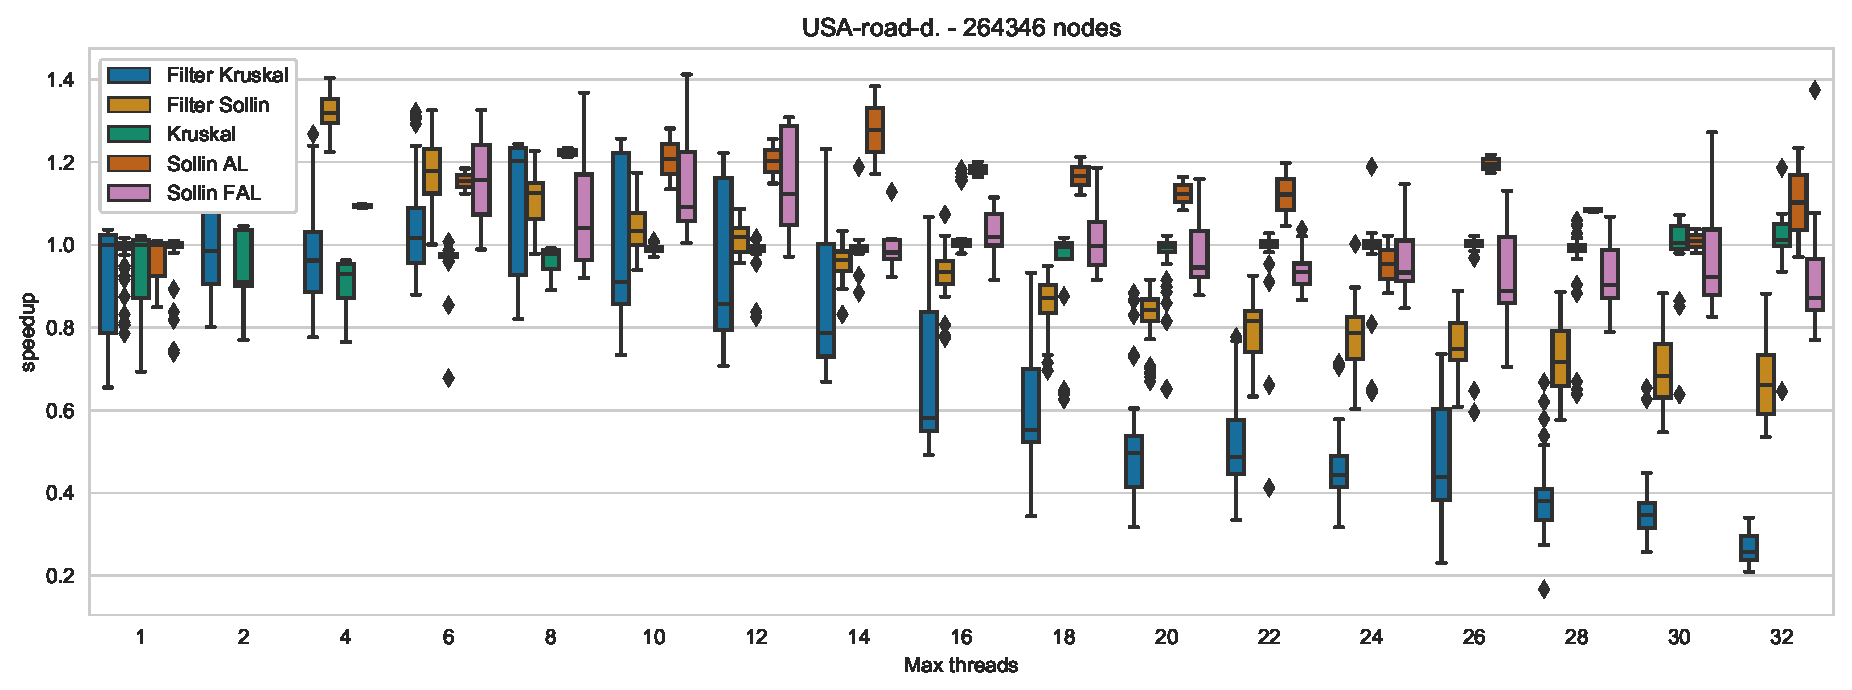
\includegraphics[width=\linewidth]{graphics/Box_Speedup_USA-road-d._264346.eps}
  \caption{Speedup graph on USA NY (260K nodes, 730K edges)\label{usaNYspeedup}}
\end{figure}
  
\begin{figure}\centering
  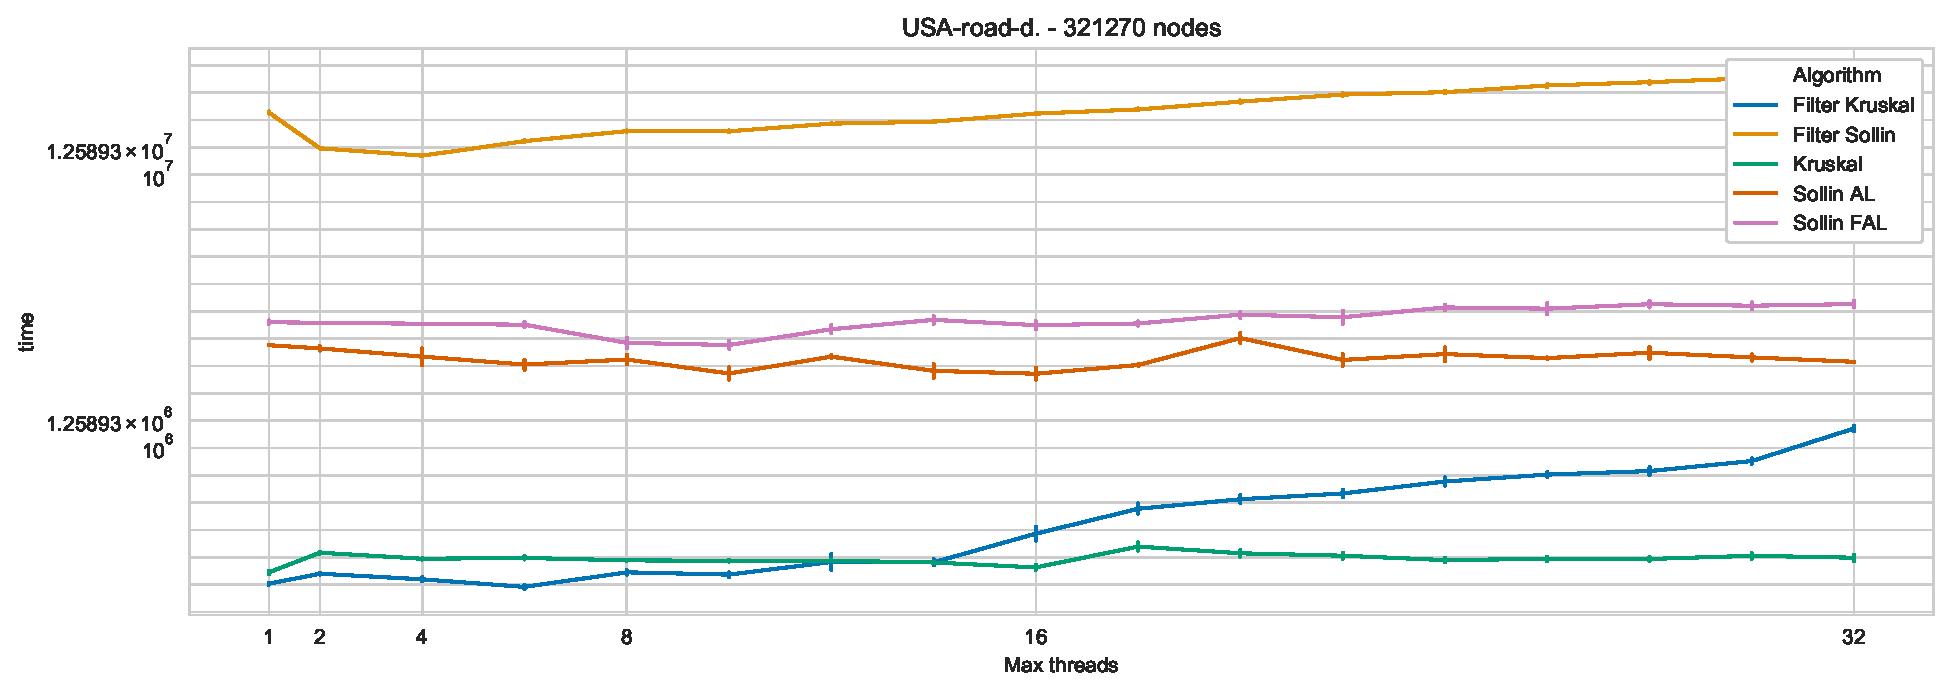
\includegraphics[width=\linewidth]{graphics/Graph_runtime_USA-road-d._321270.eps}
  \caption{Runtime graph on USA BAY (320K nodes, 800K edges)\label{usaBAYruntime}}
\end{figure}

\begin{figure}\centering
  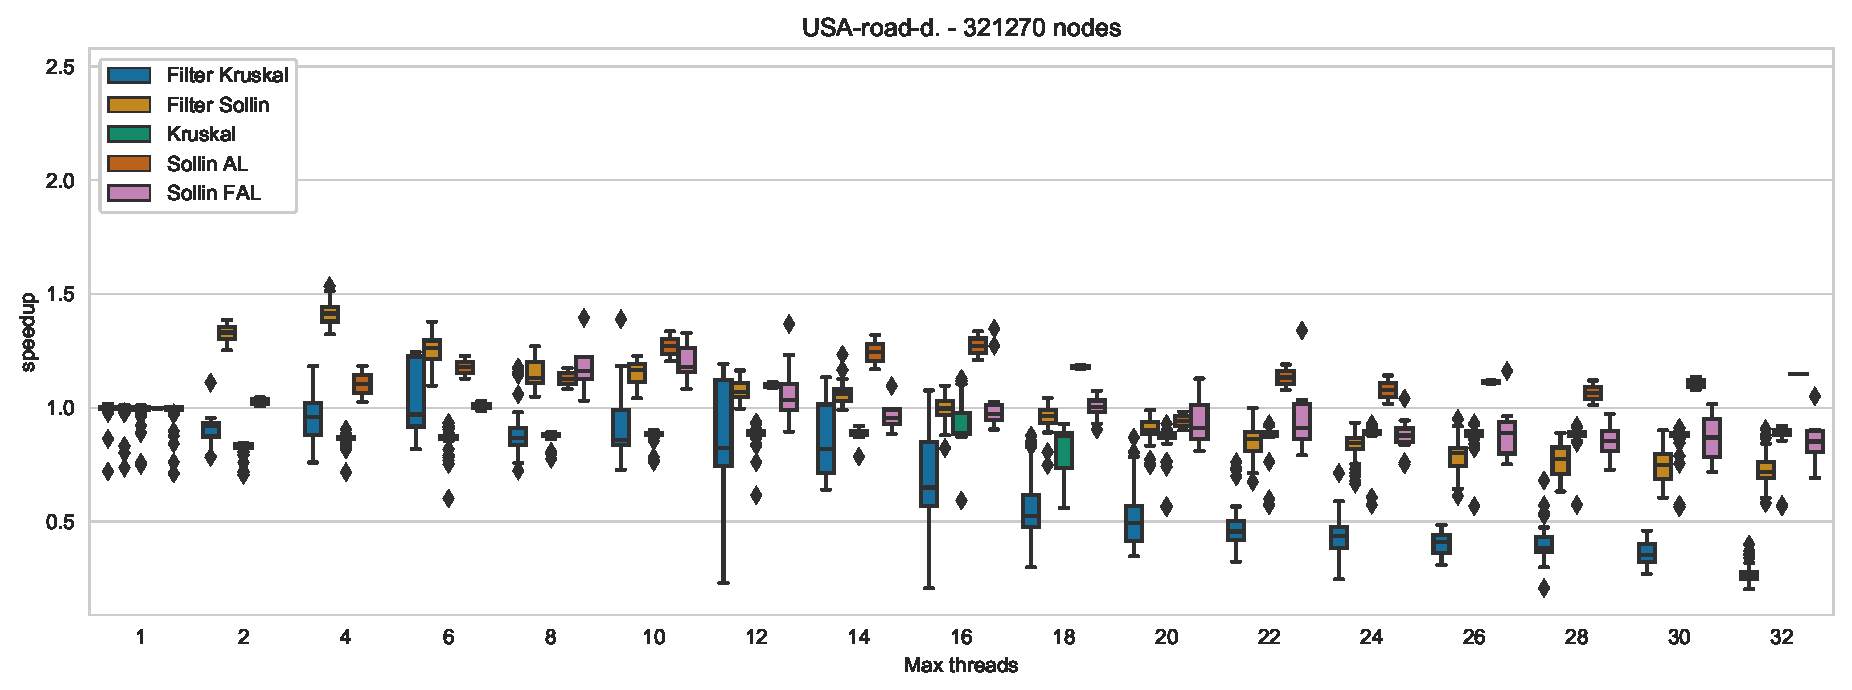
\includegraphics[width=\linewidth]{graphics/Box_Speedup_USA-road-d._321270.eps}
  \caption{Speedup graph on USA BAY (320K nodes, 800K edges)\label{usaBAYspeedup}}
\end{figure}


\subsection{Study of Amdahl's Law}

$S_p$ is the speedup with $p$ cores, $f$ is the part of the program that is sequential.

\[
        S_p = \frac{1}{\frac{1-f}{p} + f}
\]
\[
        f = \frac{\frac{p}{S_p} - 1}{p - 1}
\]

\begin{tabular}{rrrrrr}
\hline
                                                   Graph &   Filter Kruskal &   Filter Sollin &     Kruskal &   Sollin AL &   Sollin FAL \\
\hline
ER(50,000 ; 1,000) &      0.78 (0.71) &     0.42 (0.33) & 0.23 (0.21) & 0.82 (0.77) &  0.64 (0.62) \\
                  Erdos-Renyi random p=0.200000 -\ensuremath{>} 10000 &      0.96 (0.89) &     0.79 (0.73) & 0.33 (0.29) & 0.73 (0.67) &  0.88 (0.84) \\
   Preferential attachment 100 edges per vertice -\ensuremath{>} 1000 &      0.16 (0.00) &     0.00 (0.00) & 0.00 (0.00) & 0.36 (0.04) &  0.30 (0.00) \\
 Preferential attachment 1000 edges per vertice -\ensuremath{>} 10000 &      0.83 (0.81) &     0.58 (0.41) & 0.42 (0.37) &           - &  0.67 (0.56) \\
    Preferential attachment 20 edges per vertice -\ensuremath{>} 2000 &      0.00 (0.00) &     0.00 (0.00) & 0.00 (0.00) & 0.34 (0.18) &  0.00 (0.00) \\
   Preferential attachment 50 edges per vertice -\ensuremath{>} 50000 &      0.78 (0.71) &     0.21 (0.17) & 0.28 (0.26) & 0.65 (0.60) &  0.55 (0.47) \\
                                   USA-road-d. -\ensuremath{>} 264346 &      0.19 (0.00) &     0.43 (0.00) & 0.01 (0.00) &           - &  0.12 (0.00) \\
                                   USA-road-d. -\ensuremath{>} 321270 &      0.00 (0.00) &     0.50 (0.00) & 0.00 (0.00) &           - &  0.17 (0.00) \\
\hline
\end{tabular}


\section{Conclusions}

We implemented five parallel algorithms for computing a minimum spanning tree in a connected graph based on Kruskal's and Sollin's greedy approaches.

From testing them on various benchmarks (dense graphs, sparse graphs and real-life graphs), we observed that the Minimum Spanning Tree problem is particularly hard to parallelise as it is inherently sequential. 

Moreover, the performance of the algorithms largely depends upon the topology of the input graphs : PA graphs have structures much more unequally distributed than ER graphs and, therefore, lead to inferior speedups. On the graphs from the USA road networks dataset that have a even less regular topology, the algorithms do not scale at all.

Globally, on the different benchmarks, the best results are obtained with Filter Kruskal which benefits from the fact that all operations are done in-place.

We believe that starting from our results, it would be possible to design an algorithm that works better for a given benchmark.


\clearpage

% References should be produced using the bibtex program from suitable
% BiBTeX files (here: bibl_conf). The IEEEbib.bst bibliography
% style file from IEEE produces unsorted bibliography list.
% -------------------------------------------------------------------------
\bibliographystyle{IEEEbib}
\bibliography{bibl_conf}

\end{document}

